%% This is an example first chapter.  You should put chapter/appendix that you
%% write into a separate file, and add a line \include{yourfilename} to
%% main.tex, where `yourfilename.tex' is the name of the chapter/appendix file.
%% You can process specific files by typing their names in at the 
%% \files=
%% prompt when you run the file main.tex through LaTeX.
\chapter{Evaluation}

With GERT, the programmer should be able to implement concurrent embedded programs
which are as performant as the equivalent C implementation, but without having to
worry about concurency abstractions and memory safety bugs. In order to evaluate GERT,
there are two questions that must be answered:

\begin{enumerate}
  \item Does GERT retain good performance despite the costs of using a High Level Language?
  \item Do the concurrency patterns of Go simplify the task of the programmer?
\end{enumerate}

The first question is addressed by benchmarks below which measure GERT's
speed in creating and responding to external events. Pin toggle (\ref{sec:pin_toggle})
measures the maximum pin toggle frequency. Interrupt response time (\ref{sec:int_time})
measures the time it takes to respond to an external interrupt. Pulse counting
(\ref{sec:pulse_count}) counts number of pulses at increasing frequencies.
Concurrent response (\ref{sec:concurrent}) measures how many external events
GERT can concurrently respond to.

The second question is harder to answer because difficulty is a subjective
measure. This thesis attemps to show that GERT presents a better framework for
concurrency through two case studies: a robot sensor platform (\ref{sec:robot})
,which runs motors and reads sensors, and a galvo laser projector (\ref{sec:laser})
which traces images onto a surface by rotating mirrors at high speeds. The case studies
present a real-world experience for using GERT.

\section{Experimental Setup} \label{sec:setup}
In all tests, GERT is run on an i.MX6Quad SOC and all measurements are taken
with a Rigol DS1054Z oscilloscope. When GERT is compared to Linux, the SOC
runs Debian 8 "Jessie" with hardfloat support. GERT is also occasionally
compared to a Teensy 3.2 microcontroller running C. The Teensy 3.2 uses a Cortex M4, which is specifically
intended for microcontroller applications, and has good real-time performance. Its event
response times represent a good comparison point for GERT and Linux. The Teensy platform
has poor concurrency support though because its Cortex M4 is a single core processor.
%%and it only has 64 kilobytes of RAM.


All of the tests make use of the GERT "embedded" package, which is an example
driver library that was developed for the i.MX6Quad. The embedded package is not intrinsic to GERT's
functionality, nor was it optimized for performance in any way. The embedded package
just aims to provide a template for how drivers can be written in the Go language.
It currently includes drivers for the UART, SPI, PWM, GIC, USDHC, GPIO, and GPT peripherals.
The embedded package also includes an implementation of the FAT32 file system, which is 
currently unused.
%%used
%%for the laser projector (\ref{sec:laser}).

%%GERT is evaluated in conditions that are representative of embedded workloads.
%%The first few tests are benchmarks which measure GERT's maximum interrupt
%%frequency and pin toggle rate. The last two tests are each case studies: a robot
%%sensor platform and a scanning-mirror galvanometer laser projector. The test SOC
%%is the Freescale i.MX6Quad. Depending on the test, it is either running assembly,
%%GERT, or Debian 8 "Jessie" with hardfloat support. A Teensy 3.2 is used for comparison
%%on a few of the latency tests because of its Cortex M4 processor. All timing
%%measurements are taken using a Rigol DS1054Z oscilloscope.

\section{Pin Toggle Frequency}\label{sec:pin_toggle}
This test measures the speed at which GERT can toggle a simple GPIO pin on
the iMX6 Quad SOC. In ARM assembly, this can be implemented in 4 lines, but compilers and 
abstractions can increase the instruction count. Higher pin
toggling frequency indicates less code in the critical path.
GERT toggles the GPIO pin by directly interfacing with the GPIO
peripheral on the iMX6, but userspace Linux code must use the
sysfs driver.
Results are shown in figure \ref{fig:toggle}.


\begin{figure} [h]
\begin{center}
  \begin{tabular}{ | l | l |}
    \hline
    Platform & Avg GPIO Toggle Rate \\ \hline
    ASM & 1.65MHz \\ \hline
    GERT Static & 568KHz \\ \hline
    Linux C & 263KHz \\ \hline
    GERT & 154KHz \\ \hline
    Linux Go & 127KHz \\
    \hline
  \end{tabular}
\end{center}
  \caption{GPIO Toggle Rates of Different Platforms}  \label{fig:toggle}
\end{figure}

%%The results show that GERT does suffer a performance decrease because of
%%Go's abstraction cost but it is not clear why GERT underperforms user-space
%%Linux C code.
%%Without all of the syscalls a user-space program must endure, there should have
%%been a speed increase.

The results of the pin toggle initially show that GERT underperforms compared to
user-space Linux C. The reason became clear after tracing GERT's execution in QEMU:
the slowdown is caused by Go's interfaces in the embedded package. The GPIO driver
in the embedded package uses Go interfaces to abstract all of the different pins.
In order to toggle a single pin with an interface requires 47 instructions:
2 function calls, 19 loads, and 11 stores. In order to increase the toggle speed,
a new static GPIO driver was developed for GERT. The new driver is just a thin layer
over the memory-mapped registers. With static device ID's, the toggled pin
can be inferred at compile time instead of run time.
The performance of the static driver is also shown in the GERT static row
of figure \ref{fig:toggle}. With a static driver, GERT is able to toggle a
pin faster than user-space C code, but it is still very slow compared to
assembly.

But what if a Linux kernel module toggled the pin instead of userland code?
Pin toggle from inside a kernel module would certainly be faster than userland
C and it would also likely be faster than GERT. Operating from within
kernel space is very dangerous though because it lacks the protections that
GERT and userspace have.

\section{Interrupt Response Time}\label{sec:int_time}
This test measures the time it takes GERT to respond to an external event
with another external event. Specifically, it is the time it takes to produce
a rising edge on a GPIO pin in response to a falling edge on a different GPIO pin.
Faster response times are important for real time control systems, such as ABS brakes
in a car.
GERT and the Teensy detect the event with hardware interrupts
but Linux polls the input pin in a tight loop because the userspace sysfs
driver does not expose interrupt attachment points.
Results are shown below in figure \ref{fig:RT}.

\begin{figure} [h]
\begin{center}
  \begin{tabular}{ | l | l |}
    \hline
    Platform & Event Reponse Time \\ \hline
    Teensy 3.2 & 1$\mu$s \\ \hline
    GERT & 6.3$\mu$s \\ \hline
    Linux C & 10$\mu$s \\ \hline
    Linux Go & 30$\mu$s \\
    \hline
  \end{tabular}
\end{center}
  \caption{Event Response Times of Different Platforms}  \label{fig:RT}
\end{figure}

The event response times follow the increasing abstraction cost for each system.
The Teensy is very fast because its interrupt controller is vectored and interrupts
do not cause a stack switch. This means that the Teensy can flip a pin within a few cycles
of receiving the interrupt. GERT is slower because the iMX6 does not have a
vectored interrupt controller, the interrupt stack must be switched, and the
interrupt handler is written in Go. When GERT gets an interrupt, it must save its
current state, decide which interrupt it received, and execute its Go handler. Despite this
complexity, the iMX6 can execute more instructions in less time because of its very
high clock rate (792MHz vs 96MHz) so it can keep up with the Teensy.

The Linux configuration is slower because external interrupts cannot directly trigger a response
from userspace. In Linux, the GPIO pins are represented by file descriptors so
IO is performed by reading/writing from the appropriate file. In response to an external interrupt,
the Linux kernel sets a flag on the file descriptor which means that there is data to read. The userspace
program does not actually see the data until it is scheduled again.

As before, a Linux kernel module would likely attain the same performance as GERT
(or even more), but would lose the benefits of a HLL.


\section{Pulse Counting}\label{sec:pulse_count}
This test measures GERT's ability to count incoming pulses. Missed pulses
indicate an excessively long interrupt handler that is still executing when the next
pulse arrives. None of the platforms were configured for re-entrant interrupt handlers
so they can all potentially miss pulses.
The pulses are provided by a Xilinx Artix 7 FPGA and they are variable in
frequency and count. The Linux benchmarks are run with polling again because the
userspace sysfs driver does not support interrupt attachment.
Results are shown in figure \ref{fig:counter}.


\begin{figure} [h]
\begin{center}
  \begin{tabular}{ | l | l | l | l |}
    \hline
    Platform & Pulse Count & Max Pulse Rate & Missed Pulses \\ \hline
    Teensy 3.2 & 10 & 2.50MHz & 2 \\ \hline
    GERT & 10 & 161KHz & 1 \\ \hline
    Linux C & 10 & 161KHz & 4 \\ \hline
    Linux Go & 10 & 50KHz & 1 \\
    \hline
  \end{tabular}
\end{center}
  \caption{Pulse Counts of Different Platforms}  \label{fig:counter}
\end{figure}

GERT and userspace Linux C achieve similar performance on this test.
Linux just missed a few pulses.

The Teensy registers more pulses than any other platform because of its
compact and efficient architecture. A dissassembly of the Cortex M4 pulse count binary
reveals a fully vectorized interrupt whose routine only contains 5
instructions and zero conditional statements.

\section{Concurrent Events}\label{sec:concurrency}
Since the iMX6 has 4 cores, GERT should be able to concurrently
register 4 interrupts. The Teensy is configured to produce 10 rising edges
at 100KHz on a single pin and GERT must concurrently register them on 4 different
GPIO pins. The sum total of registered edges should be $10\times4=40$.

Because polling is a blocking operation, a multithreaded C program that concurrently
polls 4 pins is used for this test. The multithreaded C program is also compared
to a single-threaded program.
Results are shown in figure \ref{fig:ccounter}.

\begin{figure} [h]
\begin{center}
  \begin{tabular}{ | l | l | l | l | l |}
    \hline
    Platform & Pulse Count & Pulse Rate & Min Registered & Max Registered \\ \hline
    GERT & 10 & 100KHz & 36 & 42 \\ \hline
    Linux C Multithread & 10 & 100KHz & 32 & 33 \\ \hline
    Linux C & 10 & 100KHz & 9 & 13 \\ \hline
    \hline
  \end{tabular}
\end{center}
  \caption{Concurrent Pulse Counts of Different Platforms}  \label{fig:ccounter}
\end{figure}




\section{Benchmark Conclusions}

GERT shows that it can usually outperform userspace Linux C code and it
can keep up with the Teensy in event response time. GERT also has a true interrupt
handler whereas Linux must poll due to the sysfs driver. Unfortunately, GERT
has a complicated interrupt pipeline with many conditionals so it can miss
more interrupts than the Teensy; GERT is not suitable for meeting hard deadlines.

GERT and Linux have similar concurrent capabilities. When the frequency of external
events exceeds the response time of a single core, the events can be split among
multiple cores. In GERT, though, this threshold frequency is about 4$\mu$s faster
so the programmer can avoid dedicating additional cores in some cases.


The Go garbage collector was never an issue during any of the tests because the
benchmark programs were all static. Without memory to reclaim, the GC never
had to run. However, if the GC did run, the only test that would have been affected is
the pin toggle test because the GC is allowed to stop the world. In GERT, interrupts
can trigger even when the world is stopped so the GC will not affect the response time
and pulse counting benchmarks even though it would affect them in the Linux Go benchmarks.

\section{Case Study: Robot Sensor Platform} \label{sec:robot}

\begin{figure}[h]
  \begin{center}
 \end{center}
  \caption{Code Breakdown of Robot Sensor Platform} \label{fig:robot_code}
\end{figure}

In order to evaluate GERT on a realistic workload, I put it on a robot that was
donated to me from MIT's MASLAB competition. Among other things, the robot has two drive
motors with encoders and also several Sharp GP2Y0A21YK infrared distance sensors on its perimeter.
I wrote a program in Go using GERT to process all of these event sources at the same time
and operate the robot.

\subsection{Overview}
The main body of the robot program is an event loop which waits for events coming out of an event channel (fig. \ref{fig:event_loop}).
Independent goroutines monitor each sensor and send events into the event channel. There is a
single goroutine that monitors the event channel and manipulates state in a non-blocking manner. The code for the
event loop is shown below in fig. \ref{fig:event_loop}.

\begin{figure}[h]
  \begin{center}
\begin{lstlisting}
select {
	case event := <-event_chan:
		fmt.Printf("%v\n", event)
		switch event {
		case "p":
			val := adc.Read(0)
			fmt.Printf("adc reads %v\n", val)
		case "w":
			drive.Forward(0.2)
		case "s":
			drive.Backward(0.2)
		case "a":
			drive.TurnRight(0.2)
		case "d":
			drive.TurnLeft(0.2)
		case " ":
			drive.Stop()
		}
	}
\end{lstlisting}
\end{center}
  \caption{Robot Event Loop} \label{fig:event_loop}
\end{figure}

The robot program uses Go's higher order functions and closures in order to create a sensor polling helper function
as shown below in fig. \ref{fig:poll_func}. In this paradigm, every sensor gets its own goroutine which sends
data back into a central event loop.

%%\clearpage

\begin{figure}[!h]
\begin{center}
\begin{lstlisting}
type Pollfunc func() interface{}

func Poll(f Pollfunc, period time.Duration,
sink chan interface{}) chan bool {
	kill := make(chan bool)
	go func(kill chan bool) {
		for {
			select {
			case <-kill:
				return
			default:
				if period > 0 {
					time.Sleep(period)
				}
				sink <- f() //sink is usually the event channel
			}
		}
	}(kill)
	return kill
}
\end{lstlisting}
\end{center}
  \caption{Higher Order Polling Function} \label{fig:poll_func}
\end{figure}

The robot program also configured the GPIO library to use interrupts in order to count pulses on the encoder (fig. \ref{fig:encoder}).

\begin{figure}[!h]
\begin{center}
\begin{lstlisting}
embedded.WB_JP4_10.SetInput()
embedded.WB_JP4_10.EnableIntr(embedded.INTR_FALLING)
embedded.Enable_interrupt(99, 0) //send GPIO1 interrupt to CPU0
.
//go:nosplit
//go:nowritebarrierec
func irq(irqnum uint32) {
	switch irqnum {
...
	case 99:
		inc()
		embedded.ClearIntr(1)
...
	}
}
.
func inc() {
	count += 1
}

\end{lstlisting}
\end{center}
  \caption{Encoder Interrupt} \label{fig:encoder}
\end{figure}

With these powerful set of abstractions, adding events or sensors into the event loop
is simple because only a Pollfunc() must be implemented. As an added bonus, this
GERT program is automatically concurrent because the Go and GERT schedulers will
move idle cpus to any available goroutine. The rest of this case study explains how the sensors
are interfaced with GERT.


\subsection{PWM Motor Control}
The robot has an MDD10A motor speed controller for controlling the two drive motors. This device
expects a pulse-width modulated signal (PWM) on its input pins in order to direct power into the
motors. A PWM signal has a constant period and the signal is a logical "on" for part of the time
and "off" for the rest of the time (fig. \ref{fig:pwm}). The ratio of "on" time vs the period is called the duty cycle.
It is this percentage which the motor controller translates into a speed for the motor.

\begin{figure}[h]
\begin{center}
  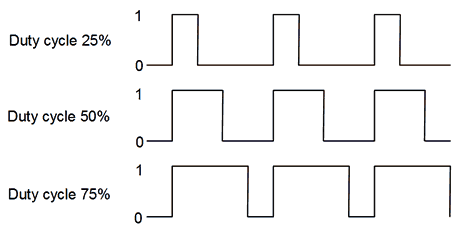
\includegraphics[scale=0.5]{pwm}
\end{center}
  \caption{Sample PWM Signals} \label{fig:pwm}
\end{figure}


The iMX6Q includes an on-board PWM peripheral which can output several channels of PWM
at a variety of periods and duty cycles. GERT contains a driver for this PWM peripheral in its embedded
package. The PWM peripheral requires no maintenance once it is configured so the cost of outputting
a PWM signal is essentially a few loads and stores every time the user changes the period or duty cycle.

The driver is organized in a typical C fashion where the memory map of the peripheral is represented in a structure:
\begin{figure}[h]
  \begin{subfigure}[t!]{0.5\textwidth}
  \begin{lstlisting}
  type PWM_regs struct {
	CR  uint32
	SR  uint32
	IR  uint32
	SAR uint32
	PR  uint32
	CNR uint32
}
  \end{lstlisting}
  \end{subfigure}
  \begin{subfigure}[t!]{0.5\textwidth}
 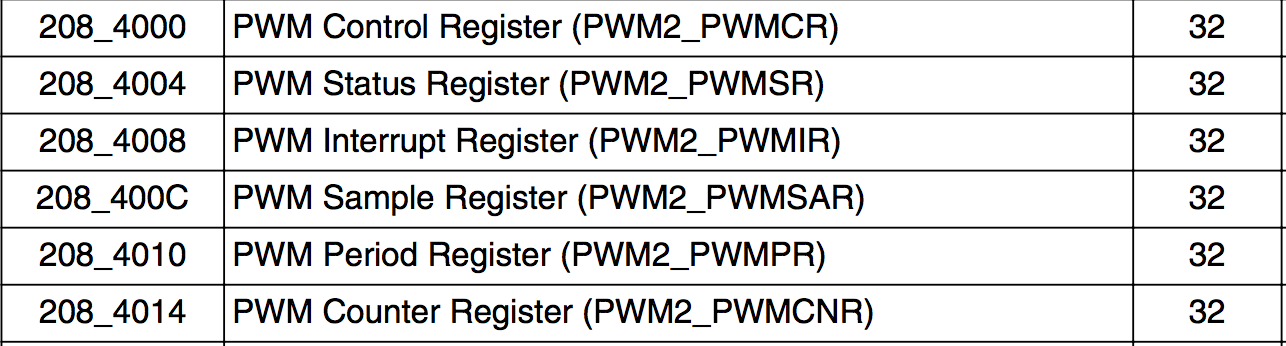
\includegraphics[scale=0.4]{pwmregs}
  \end{subfigure}
  \caption{PWM Register Representation} \label{fig:pwm_struct}
\end{figure}

The driver also exposes methods for stopping. starting, and setting the
frequency and duty cycle of the PWM generator:
\begin{figure}[h]
  \begin{lstlisting}
func (pwm *PWM_periph) Begin(freq khz)
func (pwm *PWM_periph) Stop()
func (pwm *PWM_periph) SetFreq(freq khz)
func (pwm *PWM_periph) SetDuty(dutycycle float32)
  \end{lstlisting}
  \caption{PWM Driver API} \label{fig:pwm_api}
\end{figure}

\subsection{Distance Sensor Reading}
The Sharp distance sensor outputs an analog voltage proportional to its distance from the nearest object (fig. \ref{fig:curve}).
A Microchip MCP3008 8-channel ADC is used to convert this voltage into a digital signal. The MCP3008 communicates in clocked
serial (SPI) with 24bit data frames so the robot program uses GERT's SPI driver. Much like the
PWM peripheral, the SPI peripheral has multiple channels that can each concurrently send and receive data. The SPI
driver also requires no input from the user except for the data to transmit and receive.

\begin{figure}[h]
\begin{center}
  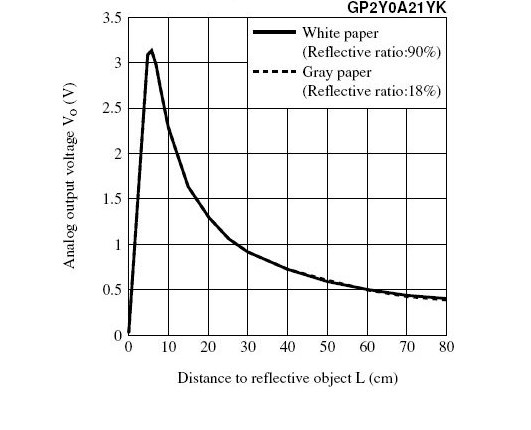
\includegraphics[scale=0.5]{IRSensor-3}
\end{center}
  \caption{Sharp Sensor Distance Curve} \label{fig:curve}
\end{figure}

\clearpage
\subsection{Encoder Reading}
Encoders emit a pulse every time the motor rotates a known amount. This amount is variable depending on the
encoder resolution. The encoders on the test motors emit pulses at a max rate of 4KHz, corresponding to
maximum motor speed. GERT had no difficulty picking up these pulses because this frequency is far less than
the max pulse frequency in fig. \ref{fig:counter}. A speed monitor was written in fig. \ref{fig:speedmon}
to measure the motor rotation (in Hz) and it corresponded very closely to the oscilliscope readings.

\begin{figure}[h]
\begin{center}
\begin{lstlisting}
//count is updated by the interrupt routine
//and it is the amount of encoder pulses
go func() {
  for {
    old := count
    time.Sleep(1 * time.Second)
    new := count
    event_chan <- new - old
  }
}()
\end{lstlisting}
\end{center}
  \caption{Motor Speed Monitor} \label{fig:speedmon}
\end{figure}

\subsection{Complications}
Systems do not work perfectly, and this robot is no exception. The switching motor controller used
on this robot emits a lot of noise. The 5v noise spikes measured on the oscilloscope wreaked havoc
on the 3.3v single-ended signals that the iMX6 operates with, causing serial communication failures
and spurious interrupts. To deal with this, the robot's motors are connected to an external power supply before
taking measurements. This helps remove noise from the digital circuits. Consequently, the physical
robot cannot move when the motors are connected to an external power supply.

\subsection{Result}
GERT is a plausible embedded toolkit to use for robots that incorporate many sensor systems.
By utilizing Go's language features, an embedded firmware engineer can implement a complicated sensor integration
platform on top of GERT without worrying about issues like scheduling or shared memory. The robot sensor platform
never experienced a single use-after-free, index out of range, or memory safety bug because it is implemented in a HLL.
As an added bonus, the robot sensor platform also does not contain a single lock despite the fact that every sensor
runs in its own thread, deadlock will never occur.



\section{Case Study: Laser Projector}\label{sec:laser}
A scanning-mirror galvanometer laser projector is a device that deflects a laser beam off of several mirrors in
order to draw an image on another surface, as shown in fig. \ref{fig:galvos}. If the entire image can be scanned faster than 24Hz, then the light appears
to blend and the human brain perceives it as a single image rather than many points. The maximum rate at which the
projector can trace points is bounded below by the speed of the galvos and bounded above by the speed of the software.
In this case study, GERT is used to implement a laser projector with a red laser.

\begin{figure}[h]
\begin{center}
  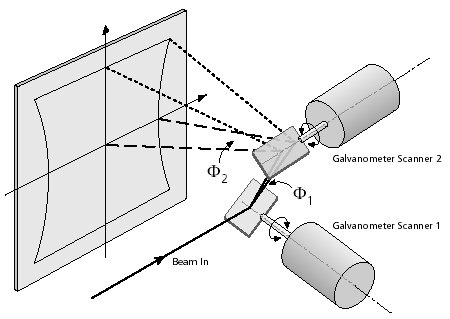
\includegraphics[scale=0.5]{galvanometer}
\end{center}
  \caption{Mirror Galvanometers} \label{fig:galvos}
\end{figure}

\subsection{Overview}
Points are generated from a vector graphics file on a desktop computer and stored
on an sdcard before GERT loads them and traces the image. The laser projector,
unlike the robot sensor platform, does not have to process any external events or
manage concurrency.
Instead, the laser program must just be fast enough to trace points smoothly.
To do this, GERT runs a dedicated goroutine, $lasermon$ which loops over all of the points
in a circular buffer and sends them in order to a Microchip MCP4922 DAC. The
DAC converts the digital position signal into an analog voltage and then
sends that voltage signal into an analog servo circuit, which sets the position
of the mirrors.

\subsection{Point Serialization}
The laser program uses Go's native Gob library in order to serialize and
deserialize points. The laser projector is currently limited to
two dimensional images with a single red laser, so only three
properties must be stored for each point: X position, Y position,
and Color. The DAC only has a 12bit resolution so 16bit integers are used
to store each point. The struct is shown below in fig. \ref{fig:cpoint}

\begin{figure}[!h]
\begin{center}
\begin{lstlisting}
type CompactPoint struct {
	X     uint16
	Y     uint16
	Color uint8 //either 0 or 1
}
\end{lstlisting}
\end{center}
  \caption{Laser Point Structure} \label{fig:cpoint}
\end{figure}

In order to store points, a seperate encoding program running
on a desktop computer encodes an array of $CompactPoint$ structs into
a Gob object and writes them to a file. Next, the encoding program stores
the file onto the FAT32-formatted sdcard that contains the GERT
program. Then, GERT reads the same file and de-serializes the Gob object
into an array of $CompactPoint$, like in fig. \ref{fig:loadpoints}.

\begin{figure}[!h]
\begin{center}
\begin{lstlisting}
	good, root := embedded.Fat32_som_start(embedded.Init_som_sdcard,
  embedded.Read_som_sdcard)
	if !good {
		fmt.Println("fat32 init failure")
	}
	good, bootdir := root.Direnter("BOOT")
	if !good {
		panic("dir entry failed")
	}
  /* P.TXT contains the Gob'ed points */
	good, contents := bootdir.Fileread("P.TXT")
	if !good {
		panic("file read failure")
	}
	r := bytes.NewBuffer(contents)
	d := gob.NewDecoder(r)
	err := d.Decode(&points)
	if err != nil {
		fmt.Printf("error de-GOBing:\n")
		panic(err)
	}
\end{lstlisting}
\end{center}
  \caption{Laser Point Structure} \label{fig:loadpoints}
\end{figure}


